\documentclass[../main.tex]{subfiles}

\begin{document}
Ovo je sekcija koju vidi samo administrator. U okviru ove sekcije, on može da doda novog zaposlenog, novu vrstu treninga, kao i novu lokaciju biranjem jedne od gornje tri opcije sa leve strane sekcije \ref{fig:administrator_novi}. Nakon što odabere operaciju, pojavljuje se odgovarajući formular, koji administrator popunjava. Nakon popunjavanja formulara, može kliknuti na dugme za čuvanje podataka u sistemu.

\begin{figure}[!ht]
\begin{center}
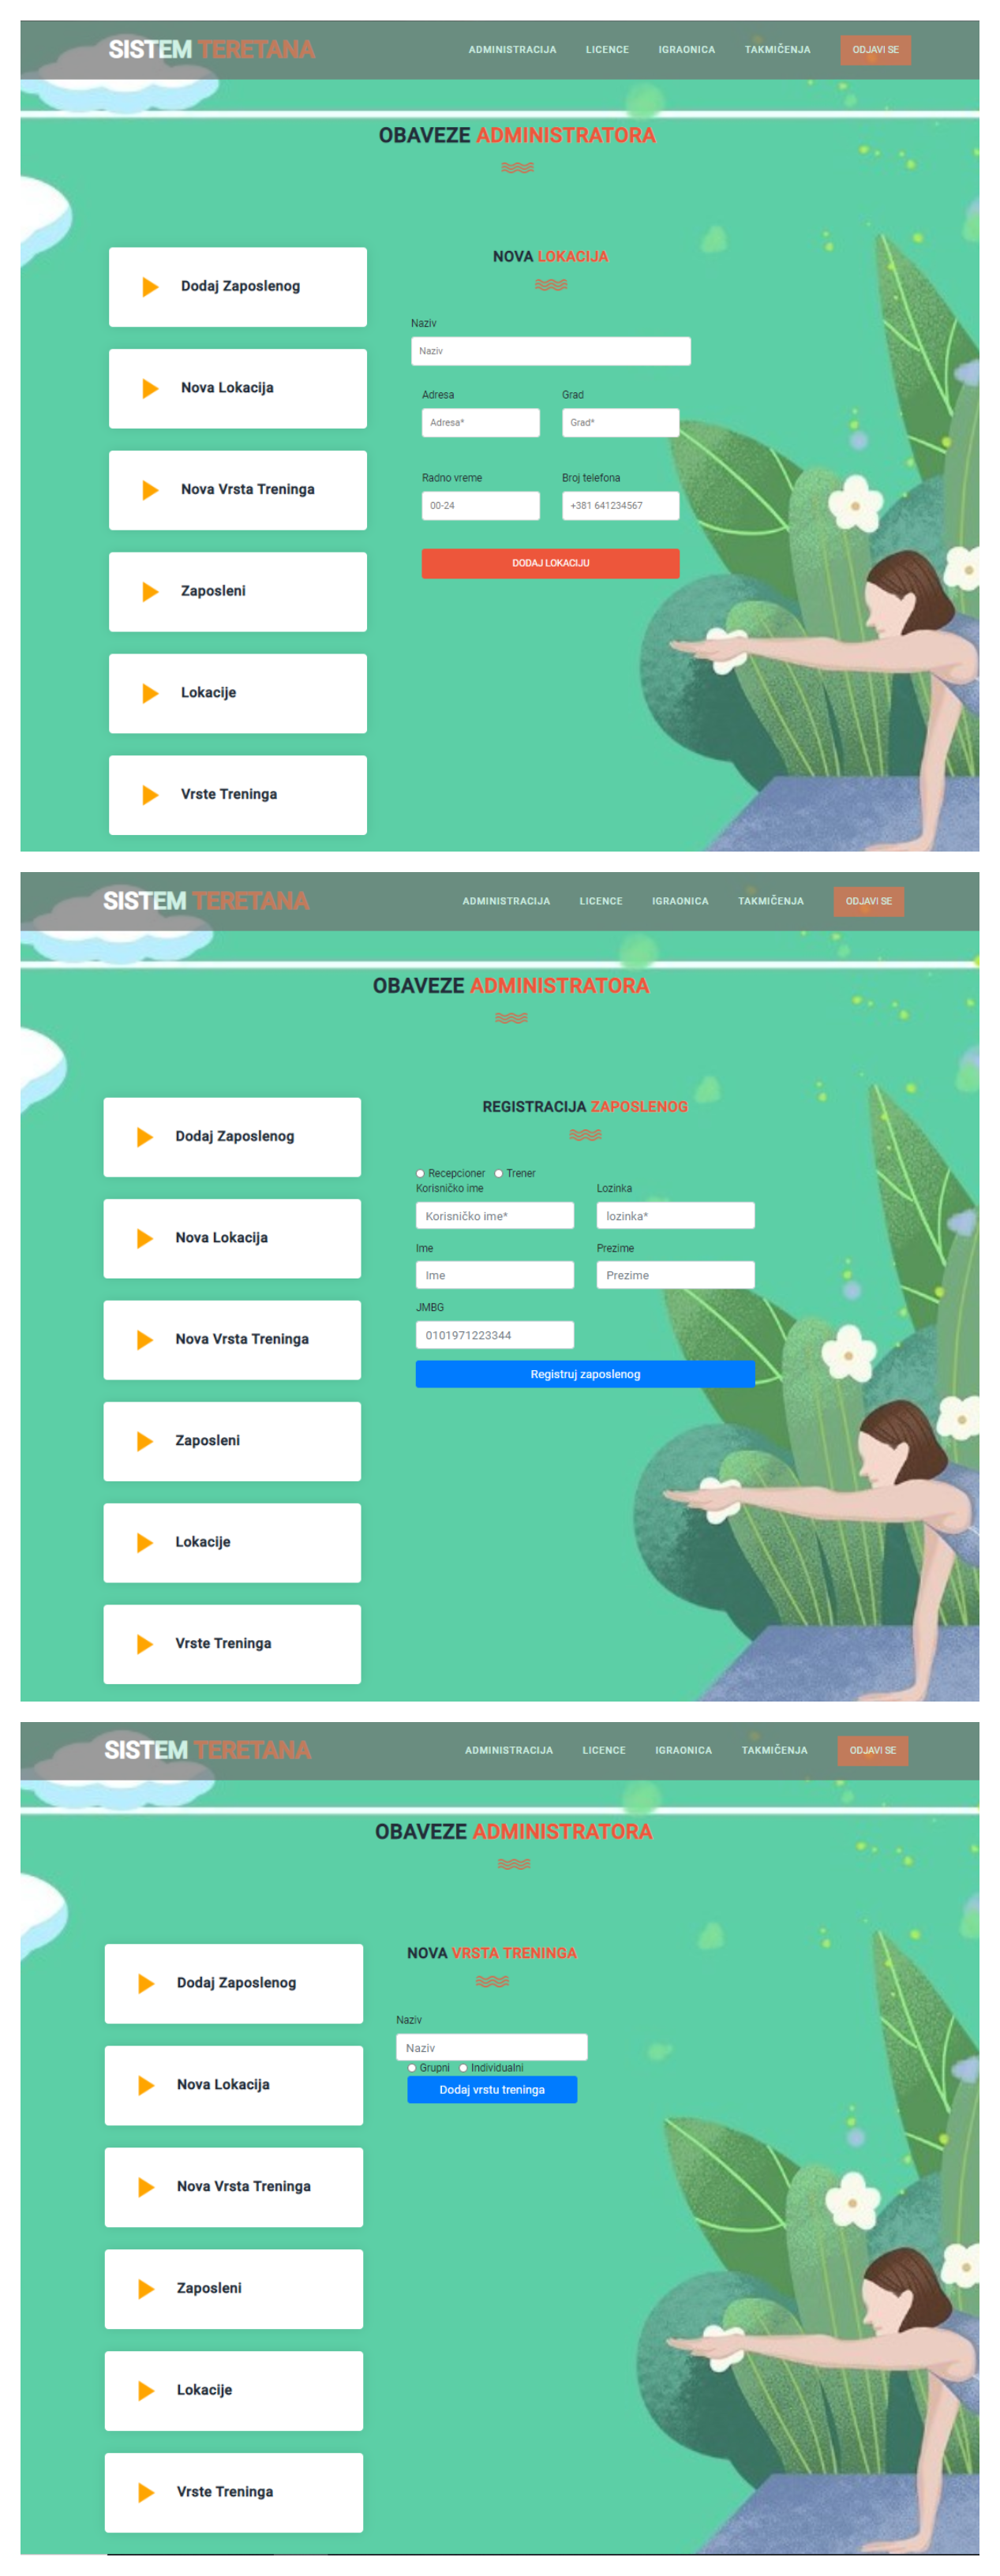
\includegraphics[scale=0.35]{sections/korisnicki_interfejs/screenshots/administrator_novi_uspravno.png}
\end{center}
\caption{Odozgo na dole: dodavanje nove lokacije, zaposlenog i vrste treninga }
\label{fig:administrator_novi}
\end{figure}

Osim toga, administrator može da pristupi i menja podatke vezane za treninge, zaposlene i lokacije teretana biranjem jedne od donje tri opcije sa leve strane sekcije \ref{fig:administrator_azuriranja}. Nakon što izabere jednu od sekcija, prikazuje se odgovarajući formular, u kojem on prvo popunjava polja za pretragu, nakon čega će se popuniti formular ispod vrednostima koje su u sistemu povezane sa vrednošću iz polja za pretragu. Nakon pregleda postojećih vrednosti, administrator može da odluči da li će i koje vrednosti menjati ili da li će iz baze obrisati sve informacije povezane sa traženim nalogom koriniska, lokacije ili vrste treninga.


\begin{figure}[!ht]
\begin{center}
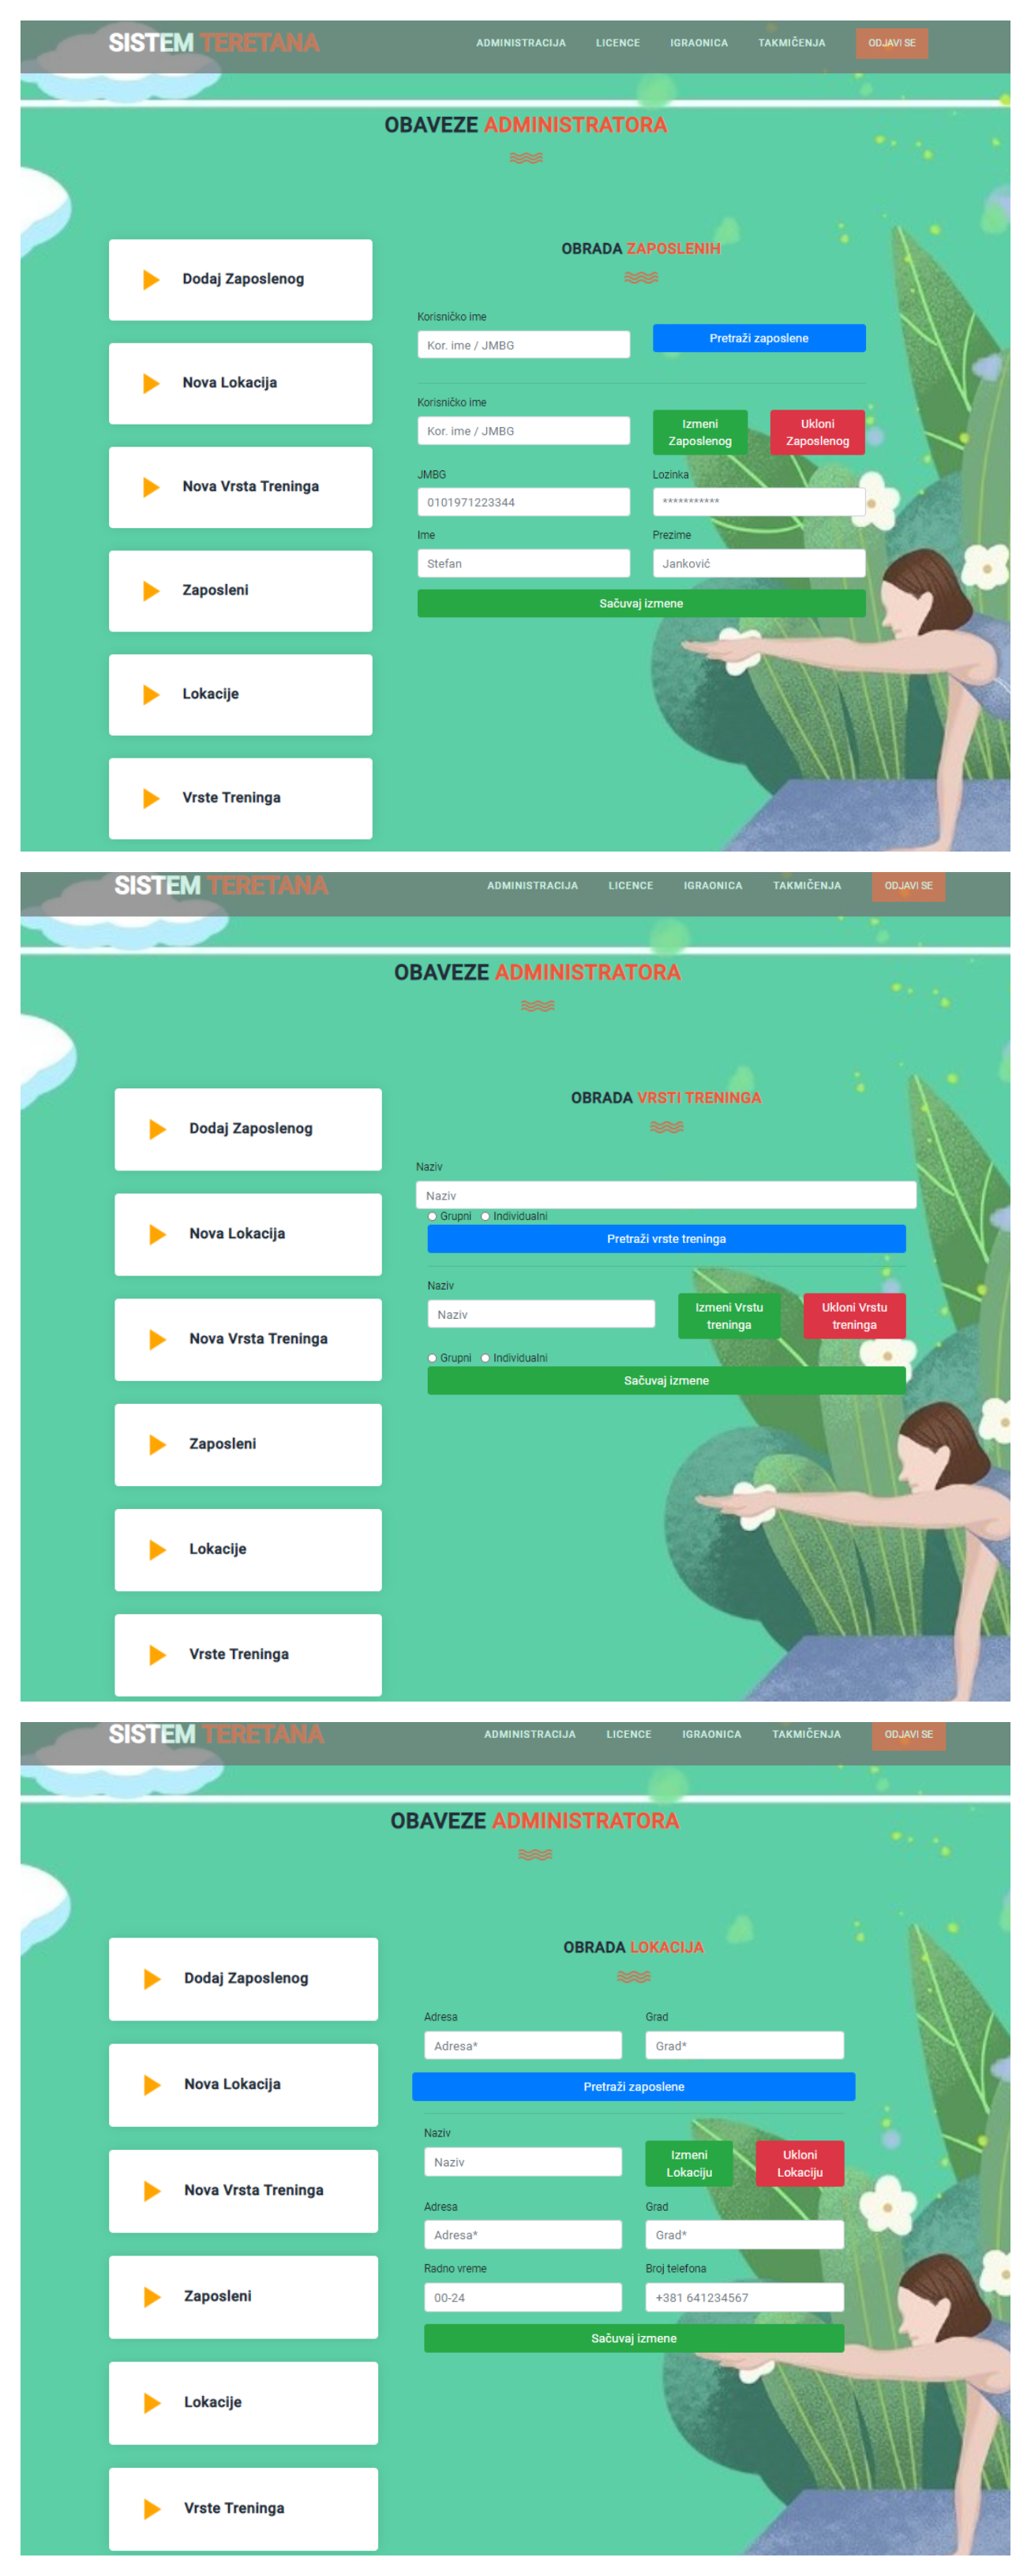
\includegraphics[scale=0.35]{sections/korisnicki_interfejs/screenshots/administrator_azuriranje.png}
\end{center}
\caption{Sleva na desno: ažuriranje i brisanje zaposlenog, vrste treninga i lokacije}
\label{fig:administrator_azuriranja}
\end{figure}



\end{document}